\documentclass{article}
\usepackage[utf8]{inputenc} % 支持UTF-8编码
\usepackage{xeCJK} % 支持中文
\usepackage{graphicx} % 引入用于插入图片的宏包
\usepackage{hyperref} % 引入超链接宏包
\usepackage{amsmath}

\usepackage{geometry}
\geometry{
  a4paper,
  left=20mm,
  right=20mm,
  top=30mm,
  bottom=30mm
}

% 设置行距为1.5倍
\usepackage{setspace}
\linespread{1.75}

\begin{document}

\title{\textbf{
GFN1000 与自然对话\\
中英双语对照翻译版
}} % 文章标题
\date{}
\maketitle % 生成标题

\setcounter{secnumdepth}{0} % 禁止章节编号,但仍添加到目录
\tableofcontents
\newpage
\section{Text 4 from On the Origin of Species/ \textit{Charles Darwin}}
\begin{center}
    CHAPTER IV\\
    NATURAL SELECTION
\end{center}

\addtolength{\leftskip}{1cm}
\addtolength{\rightskip}{1cm}

\noindent Natural Selection—its power compared with man's selection—its power on characters of trifling importance—its power at all ages and on both sexes—Sexual Selection—On the generality of intercrosses between individuals of the same species—Circumstances favourable and unfavourable to Natural Selection, namely, intercrossing, isolation, number of individuals—Slow action—Extinction caused by Natural Selection—Divergence of Character, related to the diversity of inhabitants of any small area, and to naturalisation—Action of Natural Selection, through Divergence of Character and Extinction, on the descendants from a common parent—Explains the Grouping of all organic beings.\\
第四章 自然选择——与人类选择的比较——其对不重要特征重要性的力量——在所有年龄和两性中的力量——性选择——同一物种个体间杂交的普遍性——有利于和不利于自然选择的情况,即杂交、隔离、个体数量——缓慢作用——自然选择导致的灭绝——特征的多样性,与任何小区域的居民多样性和自然化有关——自然选择的作用,通过特征的多样性和灭绝,对共同祖先的后代——解释所有生物的分类。\\

\addtolength{\leftskip}{-1cm}
\addtolength{\rightskip}{-1cm}

\noindent 1\\
How will the struggle for existence, discussed too briefly in the last chapter, act in regard to variation? Can the principle of selection, which we have seen is so potent in the hands of man, apply in nature? I think we shall see that it can act most effectually. Let it be borne in mind in what an endless number of strange peculiarities our domestic productions, and, in a lesser degree, those under nature, vary; and how strong the hereditary tendency is. Under domestication, it may be truly said that the whole organisation becomes in some degree plastic. Let it be borne in mind how infinitely complex and close-fitting are the mutual relations of all organic beings to each other and to their physical conditions of life. Can it, then, be thought improbable, seeing that variations useful to man have undoubtedly occurred, that other variations useful in some way to each being in the great and complex battle of life, should sometimes occur in the course of thousands of generations? If such do occur, can we doubt (remembering that many more individuals are born than can possibly survive) that individuals having any advantage, however slight, over others, would have the best chance of surviving and of procreating their kind? On the other hand, we may feel sure that any variation in the least degree injurious would be rigidly destroyed. This preservation of favourable variations and the rejection of injurious variations, I call Natural Selection. Variations neither useful nor injurious would not be affected by natural selection, and would be left a fluctuating element, as perhaps we see in the species called polymorphic.\\
上一章中简要讨论的生存斗争,会如何对变异产生影响呢?我们已经看到在人类手中极为有效的选择原理,能否在自然界中适用呢?我想我们将会看到,它能够极其有效地发挥作用。请记住,我们的家养生物存在着无数奇特的特性,在较小程度上,自然界中的生物也是如此,而且遗传倾向是多么强大。在驯化条件下,可以说整个生物机体在某种程度上都具有可塑性。还要记住,所有有机生物彼此之间以及它们与物质生活条件之间的相互关系是何等复杂且紧密相连。既然对人类有用的变异无疑已经出现,那么在漫长而复杂的生存斗争中,对每个生物在某些方面有用的其他变异,在数千代的过程中有时也会出现,这难道是不可想象的吗?如果确实出现了这样的变异,(请记住,出生的个体数量远远超过能够存活下来的数量)我们还能怀疑,那些比其他个体具有哪怕是最微小优势的个体,会有最好的生存和繁衍后代的机会吗?另一方面,我们可以肯定,任何哪怕是最轻微有害的变异都会被无情地淘汰。这种对有利变异的保留和对有害变异的摒弃,我称之为自然选择。既非有利也非有害的变异不会受到自然选择的影响,而会成为一种波动的因素,就像我们在所谓的多态性物种中可能看到的那样。\\ 

\noindent 2\\
We shall best understand the probable course of natural selection by taking the case of a country undergoing some physical change, for instance, of climate. The proportional numbers of its inhabitants would almost immediately undergo a change, and some species might become extinct. We may conclude, from what we have seen of the intimate and complex manner in which the inhabitants of each country are bound together, that any change in the numerical proportions of some of the inhabitants, independently of the change of climate itself, would most seriously affect many of the others. If the country were open on its borders, new forms would certainly immigrate, and this also would seriously disturb the relations of some of the former inhabitants. Let it be remembered how powerful the influence of a single introduced tree or mammal has been shown to be. But in the case of an island, or of a country partly surrounded by barriers, into which new and better adapted forms could not freely enter, we should then have places in the economy of nature which would assuredly be better filled up, if some of the original inhabitants were in some manner modified; for, had the area been open to immigration, these same places would have been seized on by intruders. In such case, every slight modification, which in the course of ages chanced to arise, and which in any way favoured the individuals of any of the species, by better adapting them to their altered conditions, would tend to be preserved; and natural selection would thus have free scope for the work of improvement.\\
我们可以通过考虑一个国家经历一些物理变化,例如气候的变化,来最好地理解自然选择的可能过程。其居民的比例数量几乎会立即发生变化,一些物种可能会灭绝。我们可以从我们所看到的每个国家的居民之间紧密而复杂的联系中得出结论,即一些居民的数量比例的任何变化,无论气候本身的改变如何,都会严重影响许多其他居民。如果该国边境开放,新的物种肯定会移民进来,这也将严重扰乱一些原有居民的关系。请记住,引入单一树种或哺乳动物的影响已被证明是强大的。但在岛屿或部分被屏障包围的国家的情况下,新的和更好的适应形式不能自由进入,我们就会在自然经济中有一些地方,如果一些原有居民以某种方式被改变,这些地方肯定会被更好地填满;因为,如果该地区对移民开放,这些地方就会被入侵者占据。在这种情况下,每一个偶然出现的微小变化,如果以任何方式有利于物种中的个体,通过更好地适应他们的改变条件,就会倾向于被保留下来;因此自然选择将有充分的空间进行改进工作。\\

\noindent 3\\
We have reason to believe, as stated in the first chapter, that a change in the conditions of life, by specially acting on the reproductive system, causes or increases variability; and in the foregoing case the conditions of life are supposed to have undergone a change, and this would manifestly be favourable to natural selection, by giving a better chance of profitable variations occurring; and unless profitable variations do occur, natural selection can do nothing. Not that, as I believe, any extreme amount of variability is necessary; as man can certainly produce great results by adding up in any given direction mere individual differences, so could Nature, but far more easily, from having incomparably longer time at her disposal. Nor do I believe that any great physical change, as of climate, or any unusual degree of isolation to check immigration, is actually necessary to produce new and unoccupied places for natural selection to fill up by modifying and improving some of the varying inhabitants. For as all the inhabitants of each country are struggling together with nicely balanced forces, extremely slight modifications in the structure or habits of one inhabitant would often give it an advantage over others; and still further modifications of the same kind would often still further increase the advantage. No country can be named in which all the native inhabitants are now so perfectly adapted to each other and to the physical conditions under which they live, that none of them could anyhow be improved; for in all countries, the natives have been so far conquered by naturalised productions, that they have allowed foreigners to take firm possession of the land. And as foreigners have thus everywhere beaten some of the natives, we may safely conclude that the natives might have been modified with advantage, so as to have better resisted such intruders.\\
我们有理由相信,正如第一章所述,生活条件的变化,通过特别作用于生殖系统,会引起或增加变异性;在前述情况下,生活条件被认为已经发生了变化,这显然有利于自然选择,因为它提供了更好的机会让有利的变异发生;除非有利的变异确实发生,否则自然选择无能为力。我并不认为,如我相信的那样,需要任何极端的变异量;正如人类可以通过在任何给定方向上累加单纯的个体差异来产生巨大的结果,大自然也可以,但更容易,因为它拥有无比更长的时间。我也不相信任何巨大的物理变化,如气候的变化,或任何不寻常的隔离程度来阻止移民,实际上都是必需的,以产生新的和未被占据的位置,供自然选择通过修改和改进一些变化的居民来填补。因为每个国家的居民都在用平衡的力量一起奋斗,一个居民的结构或习惯的极其微小的修改往往会给它带来比其他人的优势;而且同类型的进一步修改往往会进一步增加优势。没有一个国家可以被命名,其中所有的本地居民现在都如此完美地适应彼此和他们生活的物理条件,以至于他们中的任何一个都无法以任何方式得到改善;因为在所有国家,本地居民已经被归化的物种征服到如此程度,以至于他们允许外国人牢固地占有土地。由于外国人在各地都击败了一些本地居民,我们可以安全地得出结论,本地居民可能已经被有利地修改,以便更好地抵抗这些入侵者。\\

\noindent 4\\
As man can produce and certainly has produced a great result by his methodical and unconscious means of selection, what may not nature effect? Man can act only on external and visible characters: nature cares nothing for appearances, except in so far as they may be useful to any being. She can act on every internal organ, on every shade of constitutional difference, on the whole machinery of life. Man selects only for his own good; Nature only for that of the being which she tends. Every selected character is fully exercised by her; and the being is placed under well-suited conditions of life. Man keeps the natives of many climates in the same country; he seldom exercises each selected character in some peculiar and fitting manner; he feeds a long and a short beaked pigeon on the same food; he does not exercise a long-backed or long-legged quadruped in any peculiar manner; he exposes sheep with long and short wool to the same climate. He does not allow the most vigorous males to struggle for the females. He does not rigidly destroy all inferior animals, but protects during each varying season, as far as lies in his power, all his productions. He often begins his selection by some half-monstrous form; or at least by some modification prominent enough to catch his eye, or to be plainly useful to him. Under nature, the slightest difference of structure or constitution may well turn the nicely-balanced scale in the struggle for life, and so be preserved. How fleeting are the wishes and efforts of man! how short his time! and consequently how poor will his products be, compared with those accumulated by nature during whole geological periods. Can we wonder, then, that nature's productions should be far "truer" in character than man's productions; that they should be infinitely better adapted to the most complex conditions of life, and should plainly bear the stamp of far higher workmanship?\\
由于人类能够通过他有条理的无意识选择手段产生并确实产生了巨大的成果,大自然又会产生什么效果呢?人类只能作用于外部和可见的特征:大自然对外表毫不在意,除非它们对任何生物可能有用。她可以作用于每一个内部器官,每一种体质差异,整个生命机制。人类仅为自己的利益选择;大自然只为她所倾向的生物选择。每一个被选择的特征都被她充分运用;并且生物被置于适合的生活条件下。人类将许多气候的土著保持在同一个国家;他很少以某种特殊和合适的方式运用每一个被选择的特征;他用同样的食物喂养长喙和短喙的鸽子;他不会以任何特殊方式锻炼长背或长腿的四足动物;他将长毛和短毛的羊暴露在相同的气候下。他不允许最强壮的雄性为雌性而斗争。他不会严格地消灭所有劣等动物,而是在每个不同的季节里,尽其所能保护他所有的产品。他经常以某种半畸形的形式开始他的选择;或者至少以某种足够突出的修改开始,足以吸引他的目光,或对他明显有用。在大自然中,结构或体质上的最微小差异可能会很好地改变生命斗争中微妙平衡的天平,从而得以保留。人类的愿望和努力是多么短暂!他的时间是多么短暂!因此,与大自然在整个地质时期积累的产品相比,他的产品将是多么贫乏。那么,我们能不惊奇吗,大自然的产物在性格上应该比人类的产品远为“真实”;它们应该无限地更好地适应最复杂的生活条件,并明显地带有更高工艺的标志?\\

\noindent 5\\
It may be said that natural selection is daily and hourly scrutinising throughout the world, every variation, even the slightest; rejecting that which is bad, preserving and adding up all that is good; silently and insensibly working, whenever and wherever opportunity offers, at the improvement of each organic being in relation to its organic and inorganic conditions of life. We see nothing of these slow changes in progress, until the hand of time has marked the long lapse of ages, and then so imperfect is our view into long past geological ages, that we only see that the forms of life are now different from what they formerly were.\\
可以说,自然选择每天都在每时每刻审视着全世界的每一个变异,甚至是最微小的变异;淘汰坏的,保留并积累所有好的;在机会出现时,无论何时何地都在默默地、不知不觉地工作,以改善每个生物体与其有机和无机的生活条件的关系。我们看不到这些缓慢变化的进展,直到时间之手标记了漫长的岁月流逝,然后我们对遥远的地质年代的看法是如此不完美,以至于我们只看到生命的形式现在已经不同于它们以前的样子。\\

\noindent 6\\
Although natural selection can act only through and for the good of each being, yet characters and structures, which we are apt to consider as of very trifling importance, may thus be acted on. When we see leaf-eating insects green, and bark-feeders mottled-grey; the alpine ptarmigan white in winter, the red-grouse the colour of heather, and the black-grouse that of peaty earth, we must believe that these tints are of service to these birds and insects in preserving them from danger. Grouse, if not destroyed at some period of their lives, would increase in countless numbers; they are known to suffer largely from birds of prey; and hawks are guided by eyesight to their prey,—so much so, that on parts of the Continent persons are warned not to keep white pigeons, as being the most liable to destruction. Hence I can see no reason to doubt that natural selection might be most effective in giving the proper colour to each kind of grouse, and in keeping that colour, when once acquired, true and constant. Nor ought we to think that the occasional destruction of an animal of any particular colour would produce little effect: we should remember how essential it is in a flock of white sheep to destroy every lamb with the faintest trace of black. In plants the down on the fruit and the colour of the flesh are considered by botanists as characters of the most trifling importance: yet we hear from an excellent horticulturist, Downing, that in the United States smooth-skinned fruits suffer far more from a beetle, a curculio, than those with down; that purple plums suffer far more from a certain disease than yellow plums; whereas another disease attacks yellow-fleshed peaches far more than those with other coloured flesh. If, with all the aids of art, these slight differences make a great difference in cultivating the several varieties, assuredly, in a state of nature, where the trees would have to struggle with other trees and with a host of enemies, such differences would effectually settle which variety, whether a smooth or downy, a yellow or purple fleshed fruit, should succeed.\\
尽管自然选择只能通过并为了每个生物的利益而起作用,但我们倾向于认为非常微不足道的特征和结构,可能因此受到作用。当我们看到食叶昆虫是绿色的,食树皮的昆虫是斑驳的灰色;冬季的高山雷鸟是白色的,红松鸡是石楠的颜色,黑松鸡是泥炭土的颜色,我们必须相信这些颜色对这些鸟类和昆虫在保护它们免受危险方面是有帮助的。松鸡如果在它们生命中的某个时期没有被消灭,它们的数量会无限增加;它们被猛禽大量捕食;鹰是通过视力来寻找猎物的,这种视力非常敏锐,以至于在欧洲大陆的某些地方,人们被警告不要饲养白色的鸽子,因为它们最容易被捕食。因此,我看不出有任何理由怀疑自然选择可能在赋予每种松鸡适当的颜色方面最为有效,并在获得这种颜色后,保持这种颜色的真实和恒定。我们也不应该认为偶尔消灭某种特定颜色的动物会产生很小的影响:我们应该记住,在一群白色的羊中,消灭每一只带有最微弱黑色痕迹的羊羔是多么重要。在植物中,果实上的绒毛和果肉的颜色被植物学家认为是微不足道的特征:然而,我们从一位优秀的园艺学家唐宁那里听说,在美国,光滑皮肤的果实比有绒毛的果实更容易受到一种叫做象鼻虫的甲虫的侵害;紫色的李子比黄色的李子更容易受到某种疾病的侵害;而另一种疾病则对黄色果肉的桃子的侵害远大于其他颜色的果肉。如果,在所有艺术的帮助下,这些微小的差异在培育几个品种时产生了很大的差异,那么,在自然状态下,树木必须与其他树木和许多敌人作斗争,这些差异将有效地决定哪种品种,无论是光滑还是有绒毛的,黄色或紫色果肉的果实,应该成功。\\

[...]\\

\noindent 9\\
Natural selection will modify the structure of the young in relation to the parent, and of the parent in relation to the young. In social animals it will adapt the structure of each individual for the benefit of the community; if each in consequence profits by the selected change. What natural selection cannot do, is to modify the structure of one species, without giving it any advantage, for the good of another species; and though statements to this effect may be found in works of natural history, I cannot find one case which will bear investigation. A structure used only once in an animal’s whole life, if of high importance to it, might be modified to any extent by natural selection; for instance, the great jaws possessed by certain insects, and used exclusively for opening the cocoon—or the hard tip to the beak of nestling birds, used for breaking the egg. It has been asserted, that of the best short-beaked tumbler-pigeons more perish in the egg than are able to get out of it; so that fanciers assist in the act of hatching. Now, if nature had to make the beak of a full-grown pigeon very short for the bird’s own advantage, the process of modification would be very slow, and there would be simultaneously the most rigorous selection of the young birds within the egg, which had the most powerful and hardest beaks, for all with weak beaks would inevitably perish: or, more delicate and more easily broken shells might be selected, the thickness of the shell being known to vary like every other structure.\\
自然选择将根据亲代调整幼体的结构,以及根据幼体调整亲代的结构。在群居动物中,它将为群体的利益调整每个个体的结构;如果每个个体因此从所选择的变化中获益。自然选择不能做的是,在不给某一物种任何优势的情况下,为了另一物种的利益而改变其结构;尽管在自然历史作品中可以找到这种效果的陈述,但我找不到一个经得起调查的案例。一个动物一生中只使用一次的结构,如果对它非常重要,可能会被自然选择修改到任何程度;例如,某些昆虫拥有的巨大颚部,专门用于打开茧——或者雏鸟喙的硬尖,用于打破蛋壳。有人断言,最好的短喙翻飞鸽在蛋中的死亡率比能够破壳而出的要高;因此,饲养者协助孵化过程。现在,如果大自然必须为了鸟类自身的优势而使成年鸽子的喙非常短,那么修改过程将会非常缓慢,并且同时会对蛋中的幼鸟进行最严格的选择,选择那些拥有最强大和最坚硬喙的幼鸟,因为所有喙弱的都不可避免地会死亡:或者,可能会选择更精致、更容易破碎的蛋壳,因为已知蛋壳的厚度像其他任何结构一样会有所不同。\\

\noindent 10\\
\textit{Sexual Selection.}—inasmuch as peculiarities often appear under domestication in one sex and become hereditarily attached to that sex, the same fact probably occurs under nature, and if so, natural selection will be able to modify one sex in its functional relations to the other sex, or in relation to wholly different habits of life in the two sexes, as is sometimes the case with insects. And this leads me to say a few words on what I call \textit{Sexual Selection}. This depends, not on a struggle for existence, but on a struggle between the males for possession of the females; the result is not death to the unsuccessful competitor, but few or no offspring. Sexual selection is, therefore, less rigorous than natural selection. Generally, the most vigorous males, those which are best fitted for their places in nature, will leave most progeny. But in many cases, victory will depend not on general vigour, but on having special weapons, confined to the male sex. A hornless stag or spurless cock would have a poor chance of leaving offspring. Sexual selection by always allowing the victor to breed might surely give indomitable courage, length to the spur, and strength to the wing to strike in the spurred leg, as well as the brutal cock-fighter, who knows well that he can improve his breed by careful selection of the best cocks. How low in the scale of nature this law of battle descends, I know not; male alligators have been described as fighting, bellowing, and whirling round, like Indians in a war-dance, for the possession of the females; male salmons have been seen fighting all day long; male stag-beetles often bear wounds from the huge mandibles of other males. The war is, perhaps, severest between the males of polygamous animals, and these seem oftenest provided with special weapons. The males of carnivorous animals are already well armed; though to them and to others, special means of defence may be given through means of sexual selection, as the mane to the lion, the shoulder-pad to the boar, and the hooked jaw to the male salmon; for the shield may be as important for victory, as the sword or spear.\\
\textit{性选择}。—由于在圈养条件下,一些特征经常出现在一种性别中,并遗传性地附着于该性别,同样的事实可能在自然界中发生,如果是这样,自然选择将能够修改一个性别在与另一性别的功能关系中,或与两性完全不同的生活习性的关系中,就像有时昆虫的情况那样。这使我要说一些关于我所说的\textit{性选择}的话。这并不取决于生存斗争,而是取决于雄性之间为争夺雌性而进行的斗争;结果不是对失败者造成死亡,而是后代稀少或没有。因此,性选择比自然选择不那么严格。一般来说,最强壮的雄性,那些最适合它们在自然界中的位置的,将留下最多的后代。但在许多情况下,胜利将不取决于一般活力,而取决于拥有仅限于雄性的特殊武器。没有角的雄鹿或没有距的公鸡留下后代的机会很小。性选择总是允许胜利者繁殖,肯定可以赋予无可战胜的勇气,距的长度,以及在距腿上打击的翅膀的力量,以及残忍的斗鸡者,他很清楚他可以通过仔细选择最好的公鸡来改善他的品种。这种战斗法则在自然界的尺度上下降到多低,我不知道;有人描述雄性短吻鳄为争夺雌性而战斗、咆哮和旋转,就像印第安人的战舞;有人看到雄性鲑鱼整天战斗;雄性鹿角甲虫常常带着其他雄性巨大颚部造成的伤口。战争可能在一夫多妻制动物的雄性之间最为激烈,这些动物似乎最常配备特殊武器。食肉动物的雄性已经很好地武装起来;尽管对它们和对其他动物,可以通过性选择手段获得特殊的防御手段,如狮子的鬃毛、野猪的肩垫和雄性鲑鱼的钩状颚;因为盾牌对于胜利可能和剑或矛一样重要。\\

\noindent 11\\
Amongst birds, the contest is often of a more peaceful character. All those who have attended to the subject, believe that there is the severest rivalry between the males of many species to attract by singing the females. The rock-thrush of Guiana, birds of Paradise, and some others, congregate; and successive males display their gorgeous plumage and perform strange antics before the females, which standing by as spectators, at last choose the most attractive partner. Those who have closely attended to birds in confinement well know that they often take individual preferences and dislikes: thus Sir R. Heron has described how one pied peacock was eminently attractive to all his hen birds. It may appear childish to attribute any effect to such apparently weak means: I cannot here enter on the details necessary to support this view; but if man can in a short time give elegant carriage and beauty to his bantams, according to his standard of beauty, I can see no good reason to doubt that female birds, by selecting, during thousands of generations, the most melodious or beautiful males, according to their standard of beauty, might produce a marked effect. I strongly suspect that some well-known laws with respect to the plumage of male and female birds, in comparison with the plumage of the young, can be explained on the view of plumage having been chiefly modified by sexual selection, acting when the birds have come to the breeding age or during the breeding season; the modifications thus produced being inherited at corresponding ages or seasons, either by the males alone, or by the males and females; but I have not space here to enter on this subject.\\
在鸟类中,竞争往往具有更和平的性质。所有关注这一主题的人都相信,许多物种的雄性之间存在着最激烈的竞争,以歌声吸引雌性。圭亚那的岩鸫、天堂鸟和其他一些鸟类会聚集在一起;连续的雄性在雌性面前展示它们华丽的羽毛并表演奇怪的动作,雌性则作为旁观者站在一旁,最终选择最具吸引力的伴侣。那些在圈养中仔细观察过鸟类的人很清楚,它们经常会有个人的喜好和厌恶:例如,R·赫伦爵士描述了一只杂色孔雀对他的所有雌鸟都非常有吸引力。将任何效果归因于这种表面上的微弱手段可能看起来有些幼稚:我不能在这里详细阐述支持这一观点的必要细节;但如果人类能在短时间内根据自己对美的标准赋予他的观赏鸡以优雅的举止和美丽,我看不出有任何充分的理由怀疑,雌性鸟类通过在数千代中选择最悦耳或最美丽的雄性,根据它们对美的标准,可能会产生显著的效果。我强烈怀疑,一些关于雄性和雌性鸟类羽毛与幼鸟羽毛相比的众所周知的规律,可以根据羽毛主要通过性选择进行修改的观点来解释,这种修改发生在鸟类达到繁殖年龄或繁殖季节时;由此产生的这些修改在相应的年龄或季节中被继承,无论是仅由雄性还是由雄性和雌性;但是我在这里没有空间进一步讨论这个问题。\\

\noindent 12\\
Thus it is, as I believe, that when the males and females of any animal have the same general habits of life, but differ in structure, colour, or ornament, such differences have been mainly caused by sexual selection; that is, individual males have had, in successive generations, some slight advantage over other males, in their weapons, means of defence, or charms; and have transmitted these advantages to their male offspring. Yet, I would not wish to attribute all such sexual differences to this agency: for we see peculiarities arising and becoming attached to the male sex in our domestic animals (as the wattle in male carriers, horn-like protuberances in the cocks of certain fowls, \&c.), which we cannot believe to be either useful to the males in battle, or attractive to the females. We see analogous cases under nature, for instance, the tuft of hair on the breast of the turkey-cock, which can hardly be either useful or ornamental to this bird; indeed, had the tuft appeared under domestication, it would have been called a monstrosity.\\
因此,我相信,当任何动物的雄性和雌性具有相同的一般生活习惯,但在结构、颜色或装饰上有所不同时,这些差异主要是由性选择引起的;也就是说,个别雄性在连续的世代中,相对于其他雄性在武器、防御手段或魅力方面拥有一些微小的优势;并将这些优势传递给它们的雄性后代。然而,我不希望将所有这些性别差异都归因于这种机制:因为我们在我们驯养的动物中看到一些特征出现并附着于雄性(如雄性家禽的垂肉、某些家禽公鸡的角状突起等),我们不相信这些特征对雄性在战斗中有用,或对雌性有吸引力。我们在自然界中看到类似的情况,例如,火鸡公鸡胸前的一簇毛发,这对这种鸟来说几乎不可能有用或装饰性;实际上,如果这簇毛发是在驯化下出现的,它将被称为怪物。\\

\noindent 13\\
\textit{Illustrations of the action of Natural Selection.}—In order to make it clear how, as I believe, natural selection acts, I must beg permission to give one or two imaginary illustrations. Let us take the case of a wolf, which preys on various animals, securing some by craft, some by strength, and some by fleetness; and let us suppose that the fleetest prey, a deer for instance, had from any change in the country increased in numbers, or that other prey had decreased in numbers, during that season of the year when the wolf is hardest pressed for food. I can under such circumstances see no reason to doubt that the swiftest and slimmest wolves would have the best chance of surviving, and so be preserved or selected,—provided always that they retained strength to master their prey at this or at some other period of the year, when they might be compelled to prey on other animals. I can see no more reason to doubt this, than that man can improve the fleetness of his greyhounds by careful and methodical selection, or by that unconscious selection which results from each man trying to keep the best dogs without any thought of modifying the breed.\\
\textit{自然选择作用的示例。}——为了阐明我所认为的自然选择是如何发挥作用的,我恳请允许我举一两个假想的例子。以狼为例,狼捕食各种动物,有的靠狡猾,有的靠力量,还有的靠速度;我们假设,在一年中狼最难获取食物的季节,由于环境变化,速度最快的猎物(比如鹿)数量增加了,或者其他猎物的数量减少了。在这种情况下,我毫不怀疑,速度最快、体态最轻盈的狼生存的机会最大,从而得以存活或被自然选择保留下来——前提是在一年中的这个时期或其他时期,当它们不得不捕食其他动物时,仍有足够的力量去制服猎物。我对这一点深信不疑,就如同相信人类可以通过精心且系统的选育来提高灵缇犬的速度,或者相信人们在无意改良品种的情况下,只是想饲养最好的狗,这种无意识的选择也能起到作用一样。\\

\noindent 14\\
Even without any change in the proportional numbers of the animals on which our wolf preyed, a cub might be born with an innate tendency to pursue certain kinds of prey. Nor can this be thought very improbable; for we often observe great differences in the natural tendencies of our domestic animals; one cat, for instance, taking to catch rats, another mice; one cat, according to Mr. St. John, bringing home winged game, another hares or rabbits, and another hunting on marshy ground and almost nightly catching woodcocks or snipes. The tendency to catch rats rather than mice is known to be inherited. Now, if any slight innate change of habit or of structure benefited an individual wolf, it would have the best chance of surviving and of leaving offspring. Some of its young would probably inherit the same habits or structure, and by the repetition of this process, a new variety might be formed which would either supplant or coexist with the parent-form of wolf. Or, again, the wolves inhabiting a mountainous district, and those frequenting the lowlands, would naturally be forced to hunt different prey; and from the continued preservation of the individuals best fitted for the two sites, two varieties might slowly be formed. These varieties would cross and blend where they met; but to this subject of intercrossing we shall soon have to return. I may add, that, according to Mr. Pierce, there are two varieties of the wolf inhabiting the Catskill Mountains in the United States, one with a light greyhound-like form, which pursues deer, and the other more bulky, with shorter legs, which more frequently attacks the shepherd’s flocks.\\
即使狼所捕食的各种动物的数量比例没有任何变化,狼崽出生时也可能天生就有追逐某些特定猎物的倾向。这并非是极不可能的事;因为我们经常能观察到家养动物在天性上有很大差异;例如,有的猫喜欢抓老鼠,有的猫则喜欢抓老鼠;据圣约翰先生说,有的猫会叼回有翅膀的猎物,有的会叼回野兔或家兔,还有的会在沼泽地带捕猎,几乎每晚都能抓到丘鹬或沙锥鸟。喜欢抓大鼠而非小鼠的这种倾向是可以遗传的。那么,如果任何微小的、天生的习性或身体结构上的变化对某只狼有益,那这只狼就最有可能存活下来并繁衍后代。它的一些后代可能会继承相同的习性或身体结构,通过这个过程的不断重复,可能会形成一个新的变种,这个变种要么会取代原来的狼种,要么与原来的狼种共存。再者,生活在山区的狼和生活在低地的狼,自然会被迫捕食不同的猎物;通过持续保留最适应这两种环境的个体,可能会逐渐形成两个变种。这些变种在相遇时会杂交融合;不过关于杂交这个话题,我们很快还会再讨论。我还可以补充一点,根据皮尔斯先生的说法,美国卡茨基尔山脉有两种狼,一种身形轻巧,像灵缇犬,它们追捕鹿;另一种体型更粗壮,腿较短,更常袭击牧羊人的羊群。\\

\noindent 15\\
Let us now take a more complex case. Certain plants excrete a sweet juice, apparently for the sake of eliminating something injurious from their sap: this is effected by glands at the base of the stipules in some Leguminosae, and at the back of the leaf of the common laurel. This juice, though small in quantity, is greedily sought by insects. Let us now suppose a little sweet juice or nectar to be excreted by the inner bases of the petals of a flower. In this case insects in seeking the nectar would get dusted with pollen, and would certainly often transport the pollen from one flower to the stigma of another flower. The flowers of two distinct individuals of the same species would thus get crossed; and the act of crossing, we have good reason to believe (as will hereafter be more fully alluded to), would produce very vigorous seedlings, which consequently would have the best chance of flourishing and surviving. Some of these seedlings would probably inherit the nectar-excreting power. Those individual flowers which had the largest glands or nectaries, and which excreted most nectar, would be oftenest visited by insects, and would be oftenest crossed; and so in the long-run would gain the upper hand. Those flowers, also, which had their stamens and pistils placed, in relation to the size and habits of the particular insects which visited them, so as to favour in any degree the transportal of their pollen from flower to flower, would likewise be favoured or selected. We might have taken the case of insects visiting flowers for the sake of collecting pollen instead of nectar; and as pollen is formed for the sole object of fertilisation, its destruction appears a simple loss to the plant; yet if a little pollen were carried, at first occasionally and then habitually, by the pollen-devouring insects from flower to flower, and a cross thus effected, although nine-tenths of the pollen were destroyed, it might still be a great gain to the plant; and those individuals which produced more and more pollen, and had larger and larger anthers, would be selected.\\
现在让我们来看一个更复杂的例子。某些植物会分泌一种甜汁,显然是为了从树液中排出某些有害物质:在一些豆科植物中,这是由托叶基部的腺体来完成的,而在月桂树中则是由叶子背面的腺体来完成。这种甜汁虽然量少,但却受到昆虫的极力寻觅。现在让我们假设一朵花的花瓣内侧基部会分泌少量甜汁或花蜜。在这种情况下,昆虫在寻觅花蜜时身上会沾上花粉,并且肯定会经常把花粉从一朵花带到另一朵花的柱头上。这样,同一物种的两株不同植株的花就会进行杂交;我们有充分的理由相信(后面会更全面地提及这一点),杂交行为会产生非常茁壮的幼苗,因此这些幼苗有最好的机会茁壮成长并存活下来。其中一些幼苗可能会遗传分泌花蜜的能力。那些拥有最大的腺体或蜜腺且分泌最多花蜜的花朵,会最常被昆虫光顾,也会最常进行杂交;从长远来看,它们会占据优势。此外,那些其雄蕊和雌蕊的着生位置,相对于光顾它们的特定昆虫的体型和习性,在任何程度上都有利于花粉在花朵间传播的花朵,同样也会受到青睐或被选择。我们本可以举昆虫为采集花粉而非花蜜而光顾花朵的例子;由于花粉的形成唯一目的是为了受精,所以花粉的损耗对植物来说似乎是一种纯粹的损失;然而,如果有少量花粉,一开始是偶尔地,后来则是习惯性地,被以花粉为食的昆虫从一朵花带到另一朵花,从而实现杂交,尽管十分之九的花粉被损耗了,但对植物来说可能仍然是一个巨大的收益;而那些产生越来越多花粉且花药越来越大的植株个体就会被选择出来。 

\noindent 16\\
When our plant, by this process of the continued preservation or natural selection of more and more attractive flowers, had been rendered highly attractive to insects, they would, unintentionally on their part, regularly carry pollen from flower to flower; and that they can most effectually do this, I could easily show by many striking instances. I will give only one—not as a very striking case, but as likewise illustrating one step in the separation of the sexes of plants, presently to be alluded to. Some holly-trees bear only male flowers, which have four stamens producing rather a small quantity of pollen, and a rudimentary pistil; other holly-trees bear only female flowers; these have a full-sized pistil, and four stamens with shrivelled anthers, in which not a grain of pollen can be detected. Having found a female tree exactly sixty yards from a male tree, I put the stigmas of twenty flowers, taken from different branches, under the microscope, and on all, without exception, there were pollen-grains, and on some a profusion of pollen. As the wind had set for several days from the female to the male tree, the pollen could not thus have been carried. The weather had been cold and boisterous, and therefore not favourable to bees, nevertheless every female flower which I examined had been effectually fertilised by the bees, accidentally dusted with pollen, having flown from tree to tree in search of nectar. But to return to our imaginary case: as soon as the plant had been rendered so highly attractive to insects that pollen was regularly carried from flower to flower, another process might commence. No naturalist doubts the advantage of what has been called the “physiological division of labour;” hence we may believe that it would be advantageous to a plant to produce stamens alone in one flower or on one whole plant, and pistils alone in another flower or on another plant. In plants under culture and placed under new conditions of life, sometimes the male organs and sometimes the female organs become more or less impotent; now if we suppose this to occur in ever so slight a degree under nature, then as pollen is already carried regularly from flower to flower, and as a more complete separation of the sexes of our plant would be advantageous on the principle of the division of labour, individuals with this tendency more and more increased, would be continually favoured or selected, until at last a complete separation of the sexes would be effected.\\
当我们所讨论的植物,通过对越来越具吸引力的花朵持续留存或自然选择的过程,变得对昆虫极具吸引力时,昆虫就会在无意中频繁地将花粉从一朵花带到另一朵花。而且,它们能够高效地做到这一点,我可以通过许多显著的例子轻易证明。我仅举一个例子——这个例子并非特别典型,但同样可以说明植物性别分离过程中的一个步骤,稍后会提及这一点。一些冬青树只开雄花,雄花有四枚雄蕊,产生的花粉量较少,还有一个退化的雌蕊;另一些冬青树只开雌花,雌花有发育完全的雌蕊,以及四枚花药萎缩的雄蕊,在这些萎缩的花药中检测不到一粒花粉。我发现一棵雌树与一棵雄树相距恰好六十码,我将从不同树枝上取下的二十朵雌花的柱头放在显微镜下观察,无一例外,柱头上都有花粉粒,有些柱头上甚至布满了花粉。由于连续几天风向都是从雌树吹向雄树,所以花粉不可能是被风吹来的。当时天气寒冷且狂风大作,因此不利于蜜蜂活动,然而我检查过的每一朵雌花却都被蜜蜂成功授粉了,这些蜜蜂在从一棵树飞到另一棵树寻觅花蜜时,身上意外地沾上了花粉。现在回到我们设想的情况:一旦植物对昆虫极具吸引力,使得花粉能有规律地在花朵间传播,另一个过程就可能开始了。没有博物学家会怀疑所谓 “生理分工” 的优势;因此我们可以相信,对一株植物来说,在一朵花或一整株植物上只产生雄蕊,而在另一朵花或另一株植物上只产生雌蕊,是有好处的。在人工培育且处于新环境下的植物中,有时雄性器官,有时雌性器官会或多或少地失去功能;现在如果我们设想在自然环境中也会发生哪怕极其轻微的这种情况,那么由于花粉已经有规律地在花朵间传播,而且根据分工原则,植物性别更完全的分离是有利的,那么具有这种倾向且越来越明显的个体就会不断受到青睐或被选择,直到最终实现植物性别的完全分离。 \\

\noindent 17\\
Let us now turn to the nectar-feeding insects in our imaginary case: we may suppose the plant of which we have been slowly increasing the nectar by continued selection, to be a common plant; and that certain insects depended in main part on its nectar for food. I could give many facts, showing how anxious bees are to save time; for instance, their habit of cutting holes and sucking the nectar at the bases of certain flowers, which they can, with a very little more trouble, enter by the mouth. Bearing such facts in mind, I can see no reason to doubt that an accidental deviation in the size and form of the body, or in the curvature and length of the proboscis, \&c., far too slight to be appreciated by us, might profit a bee or other insect, so that an individual so characterised would be able to obtain its food more quickly, and so have a better chance of living and leaving descendants. Its descendants would probably inherit a tendency to a similar slight deviation of structure. The tubes of the corollas of the common red and incarnate clovers (Trifolium pratense and incarnatum) do not on a hasty glance appear to differ in length; yet the hive-bee can easily suck the nectar out of the incarnate clover, but not out of the common red clover, which is visited by humble-bees alone; so that whole fields of the red clover offer in vain an abundant supply of precious nectar to the hive-bee. Thus it might be a great advantage to the hive-bee to have a slightly longer or differently constructed proboscis. On the other hand, I have found by experiment that the fertility of clover greatly depends on bees visiting and moving parts of the corolla, so as to push the pollen on to the stigmatic surface. Hence, again, if humble-bees were to become rare in any country, it might be a great advantage to the red clover to have a shorter or more deeply divided tube to its corolla, so that the hive-bee could visit its flowers. Thus I can understand how a flower and a bee might slowly become, either simultaneously or one after the other, modified and adapted to each other, by the continued preservation of individuals presenting mutual and slightly favourable deviations of structure.\\
现在让我们回到我们设想例子中的吸食花蜜的昆虫:我们可以假定,通过持续选择而使花蜜量慢慢增加的植物是一种常见植物,并且某些昆虫主要以其花蜜为食。我可以列举许多事实,来说明蜜蜂是多么急于节省时间;例如,它们有在某些花朵基部打孔并吸食花蜜的习性,而其实它们只需多费一点劲,就可以从花朵的开口处进入。考虑到这些事实,我毫不怀疑,蜜蜂身体大小和形状,或者口器的弯曲度和长度等方面的一些细微变化,细微到我们难以察觉,但可能会对蜜蜂或其他昆虫有益,这样具有这些特征的个体就能更快地获取食物,从而有更好的生存和繁衍后代的机会。其后代可能会遗传这种结构上的轻微变异倾向。普通红三叶草和绛三叶草(车轴草属的红车轴草和绛车轴草)花冠的花管,乍一看长度似乎没有区别;然而,蜜蜂能轻易地从绛三叶草中吸食花蜜,却无法从普通红三叶草中吸食,因为只有熊蜂会光顾普通红三叶草;所以大片的红三叶草田为蜜蜂提供了丰富的珍贵花蜜,但蜜蜂却无法享用。因此,对蜜蜂来说,拥有稍长一点或结构不同的口器可能会有很大的优势。另一方面,我通过实验发现,三叶草的受精情况在很大程度上取决于蜜蜂对花冠的光顾和触动,以便将花粉推到柱头表面。因此,如果在任何一个地方熊蜂变得稀少,那么对红三叶草来说,拥有更短或更深裂的花冠花管可能会有很大的优势,这样蜜蜂就能光顾它的花朵。由此我能理解,花朵和蜜蜂是如何通过持续留存那些在结构上呈现出相互且略微有利变异的个体,慢慢地同时或先后发生改变并相互适应的。\\

\noindent 18\\
I am well aware that this doctrine of natural selection, exemplified in the above imaginary instances, is open to the same objections which were at first urged against Sir Charles Lyell’s noble views on “the modern changes of the earth, as illustrative of geology;” but we now very seldom hear the action, for instance, of the coast-waves, called a trifling and insignificant cause, when applied to the excavation of gigantic valleys or to the formation of the longest lines of inland cliffs. Natural selection can act only by the preservation and accumulation of infinitesimally small inherited modifications, each profitable to the preserved being; and as modern geology has almost banished such views as the excavation of a great valley by a single diluvial wave, so will natural selection, if it be a true principle, banish the belief of the continued creation of new organic beings, or of any great and sudden modification in their structure.\\
我深知,上述假想例子中所阐述的自然选择学说,会面临与最初针对查尔斯·莱尔爵士关于 “作为地质学例证的地球近代变迁” 的卓越观点所提出的相同反对意见;但是,如今我们很少听到有人称海岸波浪的作用(例如),在涉及巨大山谷的形成或漫长内陆悬崖的塑造时,是微不足道、不值一提的原因。自然选择只能通过留存和积累极其微小的、可遗传的、对留存生物有益的变异来发挥作用;正如现代地质学几乎摒弃了诸如一次大洪水波浪就能形成一个大峡谷这样的观点一样,倘若自然选择是一条正确的原理,它也将摒弃关于新生物持续被创造出来, 或者生物结构会发生任何巨大而突然的变异这样的观念。 \\

[...]\\

\noindent 39\\
Extinction.—This subject will be more fully discussed in our chapter on Geology; but it must be here alluded to from being intimately connected with natural selection. Natural selection acts solely through the preservation of variations in some way advantageous, which consequently endure. But as from the high geometrical powers of increase of all organic beings, each area is already fully stocked with inhabitants, it follows that as each selected and favoured form increases in number, so will the less favoured forms decrease and become rare. Rarity, as geology tells us, is the precursor to extinction. We can, also, see that any form represented by few individuals will, during fluctuations in the seasons or in the number of its enemies, run a good chance of utter extinction. But we may go further than this; for as new forms are continually and slowly being produced, unless we believe that the number of specific forms goes on perpetually and almost indefinitely increasing, numbers inevitably must become extinct. That the number of specific forms has not indefinitely increased, geology shows us plainly; and indeed we can see reason why they should not have thus increased, for the number of places in the polity of nature is not indefinitely great,—not that we have any means of knowing that any one region has as yet got its maximum of species. Probably no region is as yet fully stocked, for at the Cape of Good Hope, where more species of plants are crowded together than in any other quarter of the world, some foreign plants have become naturalised, without causing, as far as we know, the extinction of any natives.\\
灭绝 —— 这个主题将在我们关于地质学的章节中更全面地讨论;但由于它与自然选择密切相关,所以在这里必须提及。自然选择仅仅通过留存某种有利的变异来发挥作用,这些变异因此得以持续存在。但是,由于所有生物都具有强大的几何级数增长能力,每个地区早已挤满了生物,因此,随着每一个被选择和青睐的物种数量增加,那些较不受青睐的物种数量就会减少并变得稀少。正如地质学告诉我们的,稀少是灭绝的先兆。我们还可以看到,任何个体数量稀少的物种,在季节波动或其天敌数量变化时,极有可能彻底灭绝。但我们还可以更进一步思考;由于新物种在持续且缓慢地产生,除非我们相信物种的数量会持续且几乎无限地增加,否则必然会有一些物种灭绝。地质学清楚地表明,物种的数量并没有无限增加;实际上,我们也能明白它们为何没有无限增加,因为自然界生态系统中的生态位数量并非无限多 —— 并不是说我们有办法知道任何一个地区是否已经达到了物种数量的最大值。可能没有任何一个\\

\noindent 40\\
Furthermore, the species which are most numerous in individuals will have the best chance of producing within any given period favourable variations. We have evidence of this, in the facts given in the second chapter, showing that it is the common species which afford the greatest number of recorded varieties, or incipient species. Hence, rare species will be less quickly modified or improved within any given period, and they will consequently be beaten in the race for life by the modified descendants of the commoner species.\\
此外,个体数量最多的物种在任何特定时期内产生有利变异的可能性最大。我们在第二章给出的事实中可以找到这方面的证据,这些事实表明,正是常见物种产生了数量最多的有记录的变种或初始物种。因此,稀有物种在任何特定时期内发生变异或进化的速度较慢,因此在生存竞争中,它们会被常见物种经过变异的后代所击败。 \\

\noindent 41\\
From these several considerations I think it inevitably follows, that as new species in the course of time are formed through natural selection, others will become rarer and rarer, and finally extinct. The forms which stand in closest competition with those undergoing modification and improvement, will naturally suffer most. And we have seen in the chapter on the Struggle for Existence that it is the most closely-allied forms,—varieties of the same species, and species of the same genus or of related genera,—which, from having nearly the same structure, constitution, and habits, generally come into the severest competition with each other. Consequently, each new variety or species, during the progress of its formation, will generally press hardest on its nearest kindred, and tend to exterminate them. We see the same process of extermination amongst our domesticated productions, through the selection of improved forms by man. Many curious instances could be given showing how quickly new breeds of cattle, sheep, and other animals, and varieties of flowers, take the place of older and inferior kinds. In Yorkshire, it is historically known that the ancient black cattle were displaced by the long-horns, and that these “were swept away by the short-horns” (I quote the words of an agricultural writer) “as if by some murderous pestilence.”\\
基于上述几点考虑,我认为必然会得出这样的结论:随着时间推移,新物种通过自然选择不断形成,其他物种则会变得越来越稀少,最终走向灭绝。与那些正在经历变异和进化的物种竞争最为激烈的生物类型,自然会受到最大的冲击。我们在关于 “生存斗争” 的章节中已经了解到,亲缘关系最为密切的生物类型 —— 同一物种的变种,以及同一属或相关属的物种,由于它们的结构、体质和习性几乎相同,通常会彼此展开最为激烈的竞争。因此,每一个新变种或新物种在形成过程中,通常会对与其亲缘关系最近的物种构成最大的压力,并趋于将它们灭绝。我们在人工培育的产物中也能看到同样的灭绝过程,人类会选择改良的品种。可以列举出许多有趣的例子,表明牛、羊及其他动物的新品种,以及花卉的变种,能够多么迅速地取代旧有的、品质较差的种类。在约克郡,从历史记载可知,古代的黑牛被长角牛所取代,而长角牛 “又被短角牛淘汰”(我引用一位农业作家的话),“就好像遭受了某种致命的瘟疫一样” 。 \\

\noindent 42\\
Divergence of Character.—The principle, which I have designated by this term, is of high importance on my theory, and explains, as I believe, several important facts. In the first place, varieties, even strongly-marked ones, though having somewhat of the character of species—as is shown by the hopeless doubts in many cases how to rank them—yet certainly differ from each other far less than do good and distinct species. Nevertheless, according to my view, varieties are species in the process of formation, or are, as I have called them, incipient species. How, then, does the lesser difference between varieties become augmented into the greater difference between species? That this does habitually happen, we must infer from most of the innumerable species throughout nature presenting well-marked differences; whereas varieties, the supposed prototypes and parents of future well-marked species, present slight and ill-defined differences. Mere chance, as we may call it, might cause one variety to differ in some character from its parents, and the offspring of this variety again to differ from its parent in the very same character and in a greater degree; but this alone would never account for so habitual and large an amount of difference as that between varieties of the same species and species of the same genus.\\
性状分异 —— 我用这个术语所指的原理,在我的理论中极为重要,而且我相信,它可以解释几个重要的事实。首先,变种,即使是特征明显的变种,尽管在某种程度上具有物种的特征(这从在许多情况下难以确定如何对它们进行分类就可以看出),但它们彼此之间的差异肯定远小于明确的不同物种之间的差异。然而,在我看来,变种是正在形成过程中的物种,或者如我所称的,是初始物种。那么,变种之间较小的差异是如何扩大为物种之间较大的差异的呢?我们必然会从自然界中无数呈现出明显差异的物种推断出,这种情况是经常发生的;而变种,作为未来特征明显的物种的假定原型和亲本,只呈现出细微且不明确的差异。我们所谓的纯粹偶然因素,可能会使一个变种在某些特征上与其亲本不同,而这个变种的后代又会在同一特征上与亲本有更大程度的差异;但仅凭这一点,永远无法解释同一物种的变种之间以及同一属的物种之间如此常见且巨大的差异。 

\noindent 43\\
As has always been my practice, let us seek light on this head from our domestic productions. We shall here find something analogous. A fancier is struck by a pigeon having a slightly shorter beak; another fancier is struck by a pigeon having a rather longer beak; and on the acknowledged principle that “fanciers do not and will not admire a medium standard, but like extremes,” they both go on (as has actually occurred with tumbler-pigeons) choosing and breeding from birds with longer and longer beaks, or with shorter and shorter beaks. Again, we may suppose that at an early period one man preferred swifter horses; another stronger and more bulky horses. The early differences would be very slight; in the course of time, from the continued selection of swifter horses by some breeders, and of stronger ones by others, the differences would become greater, and would be noted as forming two sub-breeds; finally, after the lapse of centuries, the sub-breeds would become converted into two well-established and distinct breeds. As the differences slowly become greater, the inferior animals with intermediate characters, being neither very swift nor very strong, will have been neglected, and will have tended to disappear. Here, then, we see in man’s productions the action of what may be called the principle of divergence, causing differences, at first barely appreciable, steadily to increase, and the breeds to diverge in character both from each other and from their common parent.\\
就像我一直以来的做法一样,让我们从家养生物中寻找关于这个问题的启示。我们会在这里发现一些类似的情况。一位养鸽爱好者注意到一只喙略短的鸽子;另一位爱好者则注意到一只喙较长的鸽子;根据 “养鸽者不欣赏也不会欣赏中等标准,而是喜欢极端特征” 这一公认原则,他们都会继续(就像在翻飞鸽中实际发生的那样)选择喙越来越长或越来越短的鸽子进行繁育。同样,我们可以设想,在早期,一个人喜欢速度更快的马,另一个人则喜欢更强壮、体型更大的马。最初的差异会非常小;随着时间的推移,一些育种者持续选择速度更快的马,而另一些人选择更强壮的马,差异就会变得更大,并逐渐形成两个亚品种;最终,几个世纪后,这些亚品种会演变成两个成熟且截然不同的品种。随着差异慢慢增大,那些具有中间特征的、既不是特别快也不是特别强壮的劣质马匹就会被忽视,并趋于消失。因此,在这里,我们在家养生物中看到了所谓 “性状分异原理” 的作用,它使起初几乎难以察觉的差异稳步增大,并且使各个品种在特征上彼此不同,也与它们的共同祖先不同。 \\

\noindent 44\\
But how, it may be asked, can any analogous principle apply in nature? I believe it can and does apply most efficiently, from the simple circumstance that the more diversified the descendants from any one species become in structure, constitution, and habits, by so much will they be better enabled to seize on many and widely diversified places in the polity of nature, and so be enabled to increase in numbers.\\
但可能有人会问,类似的原理如何能在自然界中适用呢?我相信它能够而且确实能极为有效地适用,原因很简单,任何一个物种的后代在结构、体质和习性上变得越多样化,它们就越能更好地占据自然界生态系统中众多且差异极大的生态位,从而数量得以增加。 \\

\noindent 45\\
We can clearly see this in the case of animals with simple habits. Take the case of a carnivorous quadruped, of which the number that can be supported in any country has long ago arrived at its full average. If its natural powers of increase be allowed to act, it can succeed in increasing (the country not undergoing any change in its conditions) only by its varying descendants seizing on places at present occupied by other animals: some of them, for instance, being enabled to feed on new kinds of prey, either dead or alive; some inhabiting new stations, climbing trees, frequenting water, and some perhaps becoming less carnivorous. The more diversified in habits and structure the descendants of our carnivorous animal became, the more places they would be enabled to occupy. What applies to one animal will apply throughout all time to all animals—that is, if they vary—for otherwise natural selection can do nothing. So it will be with plants. It has been experimentally proved, that if a plot of ground be sown with one species of grass, and a similar plot be sown with several distinct genera of grasses, a greater number of plants and a greater weight of dry herbage can thus be raised. The same has been found to hold good when first one variety and then several mixed varieties of wheat have been sown on equal spaces of ground. Hence, if any one species of grass were to go on varying, and those varieties were continually selected which differed from each other in at all the same manner as distinct species and genera of grasses differ from each other, a greater number of individual plants of this species of grass, including its modified descendants, would succeed in living on the same piece of ground. And we well know that each species and each variety of grass is annually sowing almost countless seeds; and thus, as it may be said, is striving its utmost to increase its numbers. Consequently, I cannot doubt that in the course of many thousands of generations, the most distinct varieties of any one species of grass would always have the best chance of succeeding and of increasing in numbers, and thus of supplanting the less distinct varieties; and varieties, when rendered very distinct from each other, take the rank of species.\\
我们可以从习性简单的动物身上清楚地看到这一点。以一种肉食性的四足动物为例,在任何一个地区,其能够维持的数量早已达到了平均饱和水平。如果让它的自然繁殖能力发挥作用,在该地区环境条件不发生任何变化的情况下,它要增加数量,只能通过其变异的后代占据目前其他动物所占据的生态位:例如,它们中的一些能够以新的猎物为食,无论是死的还是活的;一些栖息在新的环境中,比如爬树、靠近水源,还有一些可能变得不那么肉食性。这种肉食性动物的后代在习性和结构上变得越多样化,它们能够占据的生态位就越多。适用于一种动物的情况,在任何时候对所有动物都适用 —— 也就是说,如果它们发生变异的话,否则自然选择将无法发挥作用。植物的情况也是如此。实验证明,如果在一块土地上播种一个草种,而在另一块相似的土地上播种几个不同属的草种,后者能够生长出更多的植株和更重的干草。当在同等面积的土地上先播种一个小麦变种,然后播种几个混合的小麦变种时,也发现了同样的情况。因此,如果任何一个草种持续发生变异,并且那些彼此之间的差异与不同草种和草属之间的差异相同的变种被不断选择出来,那么这个草种包括其变异后代在内的更多个体植株,就能在同一块土地上生存下来。我们都知道,每个草种和每个草的变种每年都会播撒几乎数不清的种子,可以说,它们都在竭尽全力地增加数量。因此,我毫不怀疑,在数千代的过程中,任何一个草种中差异最显著的变种总是最有机会成功生存并增加数量,从而取代差异不那么显著的变种;而当变种之间的差异变得非常明显时,它们就成为了不同的物种。\\ 

\noindent 46\\
The truth of the principle, that the greatest amount of life can be supported by great diversification of structure, is seen under many natural circumstances. In an extremely small area, especially if freely open to immigration, and where the contest between individual and individual must be severe, we always find great diversity in its inhabitants. For instance, I found that a piece of turf, three feet by four in size, which had been exposed for many years to exactly the same conditions, supported twenty species of plants, and these belonged to eighteen genera and to eight orders, which shows how much these plants differed from each other. So it is with the plants and insects on small and uniform islets; and so in small ponds of fresh water. Farmers find that they can raise most food by a rotation of plants belonging to the most different orders: nature follows what may be called a simultaneous rotation. Most of the animals and plants which live close round any small piece of ground, could live on it (supposing it not to be in any way peculiar in its nature), and may be said to be striving to the utmost to live there; but, it is seen, that where they come into the closest competition with each other, the advantages of diversification of structure, with the accompanying differences of habit and constitution, determine that the inhabitants, which thus jostle each other most closely, shall, as a general rule, belong to what we call different genera and orders.\\
结构的高度多样化能够维持最多生命数量这一原理的正确性,在许多自然环境中都能得到体现。在一个极其狭小的区域内,尤其是在对迁入没有限制且个体之间竞争必然激烈的地方,我们总能发现生物种类的高度多样性。例如,我发现一块三英尺乘四英尺大小的草皮,多年来一直处于完全相同的环境条件下,却生长着二十种植物,这些植物分属于十八个属和八个目,这表明这些植物彼此之间差异很大。在小而单一的岛屿上的植物和昆虫,以及小型淡水池塘中的生物也是如此。农民们发现,通过轮种不同目的植物,能够收获最多的作物;大自然遵循的可以说是一种同时进行的 “轮作”。生活在任何一小块土地周围的大多数动植物,理论上都可以在这块土地上生存(假设这块土地没有特殊的性质),并且可以说都在竭尽全力地在那里生存;但是可以看到,在它们彼此竞争最为激烈的地方,结构多样化的优势,以及随之而来的习性和体质的差异,决定了那些彼此竞争最为激烈的生物,一般来说,分属于我们所说的不同的属和目。\\ 

[...]\\

\noindent 50\\
After the foregoing discussion, which ought to have been much amplified, we may, I think, assume that the modified descendants of any one species will succeed by so much the better as they become more diversified in structure, and are thus enabled to encroach on places occupied by other beings. Now let us see how this principle of great benefit being derived from divergence of character, combined with the principles of natural selection and of extinction, will tend to act.\\
经过上述本应进一步展开的讨论,我认为我们可以假定,任何一个物种经过变异的后代,其结构越是多样化,就越能成功,因为这样它们就能占据其他生物所占据的生态位。现在让我们看看,从性状分异中获得巨大益处的这一原理,与自然选择和灭绝原理相结合,会如何发挥作用。 \\

\noindent 51\\
The accompanying diagram will aid us in understanding this rather perplexing subject. Let A to L represent the species of a genus large in its own country; these species are supposed to resemble each other in unequal degrees, as is so generally the case in nature, and as is represented in the diagram by the letters standing at unequal distances. I have said a large genus, because we have seen in the second chapter, that on average more of the species of large genera vary than of small genera; and the varying species of the large genera present a greater number of varieties. We have, also, seen that the species, which are the commonest and the most widely-diffused, vary more than rare species with restricted ranges. Let (A) be a common, widely-diffused, and varying species, belonging to a genus large in its own country. The little fan of diverging dotted lines of unequal lengths proceeding from (A), may represent its varying offspring. The variations are supposed to be extremely slight, but of the most diversified nature; they are not supposed all to appear simultaneously, but often after long intervals of time; nor are they all supposed to endure for equal periods. Only those variations which are in some way profitable will be preserved or naturally selected. And here the importance of the principle of benefit being derived from divergence of character comes in; for this will generally lead to the most different or divergent variations (represented by the outer dotted lines) being preserved and accumulated by natural selection. When a dotted line reaches one of the horizontal lines, and is there marked by a small numbered letter, a sufficient amount of variation is supposed to have been accumulated to have formed a fairly well-marked variety, such as would be thought worthy of record in a systematic work.\\
 随附的图表将帮助我们理解这个相当复杂的主题。设A到L代表在其所在地区属于一个大属的各个物种;这些物种彼此之间的相似程度不同,这在自然界中很常见,图表中字母之间不同的间距就体现了这一点。我提到大属,是因为我们在第二章中了解到,一般来说,大属中的物种比小属中的物种更容易发生变异;而且大属中发生变异的物种会产生更多的变种。我们还看到,那些最常见、分布最广泛的物种,比分布范围有限的稀有物种更容易发生变异。设(A)是一个常见的、分布广泛且正在变异的物种,属于其所在地区的一个大属。从(A)发出的长短不一、呈扇形散开的虚线,可以代表它变异的后代。这些变异被认为极其微小,但性质极为多样;它们并非同时出现,而是往往在很长时间间隔后才出现;而且也并非都能持续相同的时间。只有那些在某种程度上有利的变异才会被保留下来,即通过自然选择得以留存。 在这里,从性状分异中获益的原理就显得至关重要;因为这通常会导致最不同或差异最大的变异(由外侧的虚线表示)被自然选择保留并积累下来。当一条虚线到达某一条水平线,并在那里标有一个带数字的小字母时,就表示已经积累了足够多的变异,从而形成了一个特征相当明显的变种,这样的变种会被认为值得在系统的著作中记录下来。 \\

\begin{figure}
    \centering
    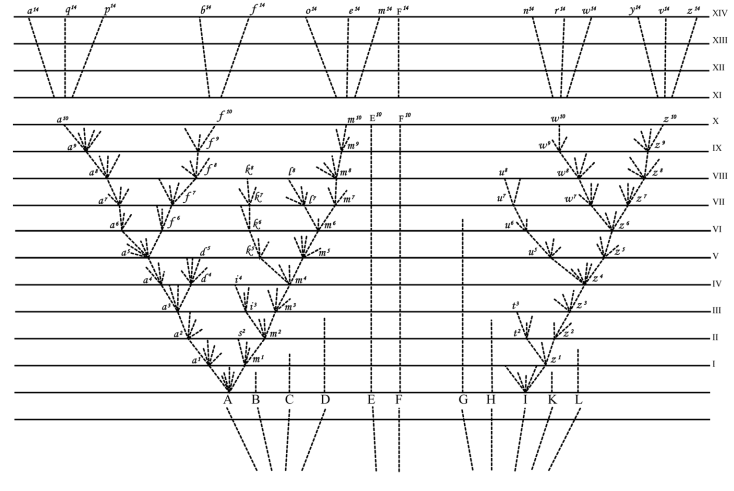
\includegraphics[width=0.75\linewidth]{image//Text4/Fig4.1.png}
\end{figure}

\noindent 52\\
The intervals between the horizontal lines in the diagram, may represent each a thousand generations; but it would have been better if each had represented ten thousand generations. After a thousand generations, species (A) is supposed to have produced two fairly well-marked varieties, namely $a^1$ and $m^1$. These two varieties will generally continue to be exposed to the same conditions which made their parents variable, and the tendency to variability is itself hereditary, consequently they will tend to vary, and generally to vary in nearly the same manner as their parents varied. Moreover, these two varieties, being only slightly modified forms, will tend to inherit those advantages which made their common parent (A) more numerous than most of the other inhabitants of the same country; they will likewise partake of those more general advantages which made the genus to which the parent-species belonged, a large genus in its own country. And these circumstances we know to be favourable to the production of new varieties.\\
图表中水平线之间的间隔,每个可以代表一千代;但如果每个间隔代表一万代可能会更好。经过一千代后,假定物种(A)产生了两个特征相当明显的变种,即$a^1$和$m^1$。这两个变种通常会继续处于使其亲代发生变异的相同环境条件下,而且变异的倾向本身是可遗传的,因此它们也会倾向于发生变异,并且通常会以与其亲代几乎相同的方式变异。此外,这两个变种只是稍有改变的形式,它们将倾向于继承那些使它们的共同亲代(A)在同一地区比大多数其他生物数量更多的优势;它们同样也会具备那些更普遍的优势,正是这些优势使得其亲代物种所属的属在该地区成为一个大属。我们知道,这些情况有利于新变种的产生。 \\

\noindent 53\\
If, then, these two varieties be variable, the most divergent of their variations will generally be preserved during the next thousand generations. And after this interval, variety $a^1$ is supposed in the diagram to have produced variety $a^2$, which will, owing to the principle of divergence, differ more from (A) than did variety $a^1$. Variety $m^1$ is supposed to have produced two varieties, namely $m^2$ and $s^2$, differing from each other, and more considerably from their common parent (A). We may continue the process by similar steps for any length of time; some of the varieties, after each thousand generations, producing only a single variety, but in a more and more modified condition, some producing two or three varieties, and some failing to produce any. Thus the varieties or modified descendants, proceeding from the common parent (A), will generally go on increasing in number and diverging in character. In the diagram the process is represented up to the ten - thousandth generation, and under a condensed and simplified form up to the fourteen thousandth generation.\\
那么,如果这两个变种是可变的,它们差异最大的变异通常会在接下来的一千代中被保留下来。在这段时间间隔后,图表中假定变种$a^1$产生了变种$a^2$,由于性状分异原理,$a^2$与(A)的差异会比$a^1$与(A)的差异更大。假定变种$m^1$产生了两个变种,即$m^2$和$s^2$,它们彼此不同,且与它们的共同亲代(A)的差异更大。我们可以按照类似的步骤将这个过程持续任意长的时间;有些变种在每一千代之后,只产生一个变种,但这个变种的变异程度越来越大;有些变种产生两到三个变种;还有一些变种则不产生任何后代。因此,从共同亲代(A)衍生出来的变种或经过变异的后代,其数量通常会不断增加,性状也会不断分异。在图表中,这个过程一直展示到了第一万代,并且以浓缩和简化的形式展示到了第一万四千代。 \\

\noindent 54\\
But I must here remark that I do not suppose that the process ever goes on so regularly as is represented in the diagram, though in itself made somewhat irregular. I am far from thinking that the most divergent varieties will invariably prevail and multiply: a medium form may often long endure, and may or may not produce more than one modified descendant; for natural selection will always act according to the nature of the places which are either unoccupied or not perfectly occupied by other beings; and this will depend on infinitely complex relations. But as a general rule, the more diversified in structure the descendants from any one species can be rendered, the more places they will be enabled to seize on, and the more their modified progeny will be increased. In our diagram the line of succession is broken at regular intervals by small numbered letters marking the successive forms which have become sufficiently distinct to be recorded as varieties. But these breaks are imaginary, and might have been inserted anywhere, after intervals long enough to have allowed the accumulation of a considerable amount of divergent variation.\\
但我必须在此指出,我并不认为这个过程会像图表中所展示的那样规则地进行,尽管图表本身已经表现得有些不规则了。我绝不是认为差异最大的变种总是会占优势并繁衍:中间形态往往可以长期存在,而且可能产生一个或多个变异后代,也可能不产生;因为自然选择总是根据那些尚未被其他生物占据,或者尚未被完全占据的生态位的性质来发挥作用,而这取决于极其复杂的关系。但一般来说,任何一个物种的后代在结构上越是多样化,它们能够占据的生态位就越多,其变异后代的数量也就会增加得越多。在我们的图表中,传承的线条会每隔一定间隔被带数字的小字母打断,这些字母标记着那些已经变得足够独特,可以被记录为变种的连续形态。但这些中断是假想的,只要间隔的时间足够长,足以积累大量的分异变异,它们可以被插入到任何地方。 \\

\noindent 55\\
As all the modified descendants from a common and widely - diffused species, belonging to a large genus, will tend to partake of the same advantages which made their parent successful in life, they will generally go on multiplying in number as well as diverging in character: this is represented in the diagram by the several divergent branches proceeding from (A). The modified offspring from the later and more highly improved branches in the lines of descent, will, it is probable, often take the place of, and so destroy, the earlier and less improved branches: this is represented in the diagram by some of the lower branches not reaching to the upper horizontal lines. In some cases I do not doubt that the process of modification will be confined to a single line of descent, and the number of the descendants will not be increased; although the amount of divergent modification may have been increased in the successive generations. This case would be represented in the diagram, if all the lines proceeding from (A) were removed, excepting that from $a^1$ to $a^{10}$. In the same way, for instance, the English race - horse and English pointer have apparently both gone on slowly diverging in character from their original stocks, without either having given off any fresh branches or races.\\
由于来自一个常见且分布广泛的物种(属于一个大属)的所有变异后代,往往会具备使其亲代在生存中取得成功的相同优势,所以它们通常在数量上会不断增加,同时在性状上也会不断分异:这在图表中表现为由(A)衍生出的几条分异的分支。在演化谱系中,来自较晚且改进程度更高分支的变异后代,很可能常常会取代并淘汰较早且改进程度较低的分支,图表中一些较低的分支没有延伸到上面的水平线就体现了这一点。在某些情况下,我毫不怀疑变异过程可能会局限于单一的演化谱系,后代的数量也不会增加,尽管在连续的世代中,分异变异的程度可能会增加。如果从(A)衍生出的所有分支中,只保留从$a^1$到$a^{10}$的这一支,而去掉其他分支,那么这种情况在图表中就能得以体现。例如,英国赛马和英国指示犬显然在性状上都从它们最初的种群开始慢慢发生分异,而且都没有产生新的分支或品种 。 \\

\noindent 56\\
After ten thousand generations, species (A) is supposed to have produced three forms, $a^{10}$, $f^{10}$, and $m^{10}$, which, from having diverged in character during the successive generations, will have come to differ largely, but perhaps unequally, from each other and from their common parent. If we suppose the amount of change between each horizontal line in our diagram to be excessively small, these three forms may still be only well - marked varieties; or they may have arrived at the doubtful category of sub - species; but we have only to suppose the steps in the process of modification to be more numerous or greater in amount, to convert these three forms into well - defined species: thus the diagram illustrates the steps by which the small differences distinguishing varieties are increased into the larger differences distinguishing species. By continuing the same process for a greater number of generations (as shown in the diagram in a condensed and simplified manner), we get eight species, marked by the letters between $a^{14}$ and $m^{14}$, all descended from (A). Thus, as I believe, species are multiplied and genera are formed.\\
经过一万代后,假定物种(A)产生了三个形态,即$a^{10}$、$f^{10}$和$m^{10}$,由于在连续的世代中性状发生了分异,它们彼此之间以及与它们的共同亲代之间会有很大的差异,但这种差异或许并不均等。如果我们假定图表中每条水平线之间的变化量极小,那么这三个形态可能仍然只是特征明显的变种;或者它们可能属于难以界定的亚种范畴;但我们只要设想变异过程中的步骤更多,或者变化量更大,就可以将这三个形态转变为明确的物种:因此,该图表展示了区分变种的微小差异是如何扩大为区分物种的较大差异的。通过将这个过程在更多世代中延续下去(如图表以浓缩和简化的方式所示),我们得到了八个物种,由$a^{14}$和$m^{14}$之间的字母表示,它们都源自(A)。因此,我认为,物种数量得以增加,属也得以形成。 \\

\noindent 57\\
In a large genus it is probable that more than one species would vary. In the diagram I have assumed that a second species (I) has produced, by analogous steps, after ten thousand generations, either two well-marked varieties ($w^{10}$ and $z^{10}$) or two species, according to the amount of change supposed to be represented between the horizontal lines. After fourteen thousand generations, six new species, marked by the letters $n^{14}$ to $z^{14}$, are supposed to have been produced. In each genus, the species, which are already extremely different in character, will generally tend to produce the greatest number of modified descendants; for these will have the best chance of filling new and widely different places in the polity of nature: hence in the diagram I have chosen the extreme species (A), and the nearly extreme species (I), as those which have largely varied, and have given rise to new varieties and species. The other nine species (marked by capital letters) of our original genus, may for a long period continue transmitting unaltered descendants; and this is shown in the diagram by the dotted lines not prolonged far upwards from want of space.\\
在一个大属中,很可能不止一个物种会发生变异。在图表中,我假定第二个物种(I)经过类似的步骤,在一万代之后,根据水平线之间所代表的变化量,产生了两个特征明显的变种($w^{10}$和$z^{10}$)或者两个物种。在一万四千代之后,假定产生了六个新物种,由字母$n^{14}$到$z^{10}$表示。在每个属中,那些在性状上已经极为不同的物种,通常倾向于产生数量最多的变异后代,因为这些后代最有机会占据自然界生态系统中新的、差异极大的生态位。因此在图表中,我选择了处于极端的物种(A),以及近乎极端的物种(I),作为发生了大量变异并产生新变种和新物种的代表。我们最初那个属中的其他九个物种(用大写字母表示),可能在很长一段时间内会继续繁衍出没有发生变化的后代,由于空间限制,图表中这些物种的虚线没有向上延伸很远来表示这一点。 \\

\noindent 58\\
But during the process of modification, represented in the diagram, another of our principles, namely that of extinction, will have played an important part. As in each fully stocked country natural selection necessarily acts by the selected form having some advantage in the struggle for life over other forms, there will be a constant tendency in the improved descendants of any one species to supplant and exterminate in each stage of descent their predecessors and their original parent. For it should be remembered that the competition will generally be most severe between those forms which are most nearly related to each other in habits, constitution, and structure. Hence all the intermediate forms between the earlier and later states, that is between the less and more improved state of a species, as well as the original parent - species itself, will generally tend to become extinct. So it probably will be with many whole collateral lines of descent, which will be conquered by later and improved lines of descent. If, however, the modified offspring of a species get into some distinct country, or become quickly adapted to some quite new station, in which child and parent do not come into competition, both may continue to exist.\\
但是在图表所展示的变异过程中,我们的另一个原理,即灭绝原理,也发挥了重要作用。在每一个物种饱和的地区,自然选择必然会使被选择的类型在生存竞争中比其他类型具有某种优势,因此任何一个物种的改进后代,在每一个演化阶段,都有取代并灭绝其祖先和原始亲代物种的趋势。应该记住,在习性、体质和结构上彼此最为相近的类型之间,竞争通常最为激烈。因此,一个物种早期和晚期状态之间,也就是较不改良和较改良状态之间的所有中间形态,以及原始亲代物种本身,通常都有灭绝的趋势。许多旁系的演化谱系很可能也是如此,它们会被后来出现且经过改良的演化谱系所取代。然而,如果一个物种的变异后代进入了某个不同的地区,或者迅速适应了某个全新的生态位,在那里子代和亲代不会产生竞争,那么两者可能都会继续生存下去。\\ 

\noindent 59\\
If then our diagram be assumed to represent a considerable amount of modification, species (A) and all the earlier varieties will have become extinct, having been replaced by eight new species ($a^{14}$ to $m^{14}$); and (I) will have been replaced by six ($n^{14}$ to $z^{14}$) new species.\\
那么,如果我们假定该图表代表了大量的变异,物种(A)和所有早期的变种将会灭绝,被八个新物种($a^{14}$到$m^{14}$)所取代;而物种(I)将会被六个($n^{14}$到$z^{14}$)新物种所取代 。 \\

\noindent 60\\
But we may go further than this. The original species of our genus were supposed to resemble each other in unequal degrees, as is so generally the case in nature; species (A) being more nearly related to B, C, and D, than to the other species; and species (I) more to G, H, K, L, than to the others. These two species (A) and (I), were also supposed to be very common and widely diffused species, so that they must originally have had some advantage over most of the other species of the genus. Their modified descendants, fourteen in number at the fourteen-thousandth generation, will probably have inherited some of the same advantages: they have also been modified and improved in a diversified manner at each stage of descent, so as to have become adapted to many related places in the natural economy of their country. It seems, therefore, to me extremely probable that they will have taken the places of, and thus exterminated, not only their parents (A) and (I), but likewise some of the original species which were most nearly related to their parents. Hence very few of the original species will have transmitted offspring to the fourteen-thousandth generation. We may suppose that only one (F), of the two species which were least closely related to the other nine original species, has transmitted descendants to this late stage of descent.\\
但我们还可以更进一步探讨。我们假定该属的原始物种彼此之间的相似程度并不相同,这在自然界中是很常见的情况;物种(A)与B、C和D的亲缘关系,比与其他物种的亲缘关系更近;而物种(I)与G、H、K、L的亲缘关系,比与其他物种的更近。这两个物种(A)和(I)也被假定为非常常见且分布广泛的物种,因此它们最初一定比该属的大多数其他物种具有某些优势。它们的变异后代在第一万四千代时有十四个,很可能继承了一些相同的优势;而且在每一个演化阶段,这些后代都以多样化的方式进行了变异和改进,从而适应了它们所在地区自然生态系统中的许多相关生态位。因此,在我看来,极有可能的是,它们不仅会取代并灭绝它们的亲代物种(A)和(I),还会取代并灭绝一些与它们亲代亲缘关系最近的原始物种。因此,很少有原始物种能够将后代繁衍到第一万四千代。我们可以假定,在与其他九个原始物种亲缘关系最不密切的两个物种中,只有一个物种(F)将后代繁衍到了这一较晚的演化阶段。\\ 

\noindent 61\\
The new species in our diagram descended from the original eleven species, will now be fifteen in number. Owing to the divergent tendency of natural selection, the extreme amount of difference in character between species $a^{14}$ and $z^{14}$ will be much greater than that between the most different of the original eleven species. The new species, moreover, will be allied to each other in a widely different manner. Of the eight descendants from (A) the three marked $a^{14}$, $q^{14}$, $p^{14}$, will be nearly related from having recently branched off from $a^{10}$; $b^{14}$ and $f^{14}$, from having diverged at an earlier period from $a^{5}$, will be in some degree distinct from the three first - named species; and lastly, $o^{14}$, $e^{14}$, and $m^{14}$, will be nearly related one to the other, but from having diverged at the first commencement of the process of modification, will be widely different from the other five species, and may constitute a sub - genus or even a distinct genus.\\
在我们的图表中,由最初的十一个物种衍生出的新物种现在有十五个。由于自然选择的分异倾向,物种$a^{14}$和$z^{14}$在性状上的极大差异,将远远大于最初十一个物种中差异最大的物种之间的差异。此外,新物种之间相互关联的方式也会大不相同。在(A)的八个后代中,标记为$a^{14}$、$q^{14}$、$p^{14}$的三个物种,因为最近才从$a^{10}$分支出来,所以亲缘关系较近;$b^{14}$和$f^{14}$由于在较早时期从$a^{5}$分异出来,在某种程度上与前面提到的三个物种不同;最后,$o^{14}$、$e^{14}$和$m^{14}$彼此之间亲缘关系较近,但由于在变异过程一开始就发生了分异,所以与其他五个物种差异很大,它们可能构成一个亚属,甚至是一个独立的属 。 \\

\noindent 62\\
The six descendants from (I) will form two sub - genera or even genera. But as the original species (I) differed largely from (A), standing nearly at the extreme points of the original genus, the six descendants from (I) will, owing to inheritance, differ considerably from the eight descendants from (A); the two groups, moreover, are supposed to have gone on diverging in different directions. The intermediate species, also (and this is a very important consideration), which connected the original species (A) and (I), have all become, excepting (F), extinct, and have left no descendants. Hence the six new species descended from (I), and the eight descended from (A), will have to be ranked as very distinct genera, or even as distinct sub - families.\\
(I)的六个后代将形成两个亚属,甚至是属。但是由于原始物种(I)与(A)差异很大,几乎处于原始属的两端,(I)的六个后代由于遗传的原因,将与(A)的八个后代有很大的差异;此外,这两个类群被认为是朝着不同的方向分异的。同样(这是一个非常重要的因素),连接原始物种(A)和(I)的中间物种,除了(F)之外,都已经灭绝,没有留下后代。因此,(I)衍生出的六个新物种和(A)衍生出的八个新物种,将被归为截然不同的属,甚至是不同的亚科。 \\

\noindent 63\\
Thus it is, as I believe, that two or more genera are produced by descent, with modification, from two or more species of the same genus. And the two or more parent - species are supposed to have descended from some one species of an earlier genus. In our diagram, this is indicated by the broken lines, beneath the capital letters, converging in sub - branches downwards towards a single point; this point representing a single species, the supposed single parent of our several new sub - genera and genera.\\
因此,我认为,两个或多个属是通过变异和遗传,从同一属的两个或多个物种演变而来的。而这两个或多个亲代物种被认为是从更早属的某个单一物种演化而来的。在我们的图表中,大写字母下方的虚线以次分支的形式向下汇聚于一个点,就表明了这一点;这个点代表一个单一物种,即我们几个新亚属和属的假定共同祖先。 \\

\noindent 68\\
Summary of Chapter.—If during the long course of ages and under varying conditions of life, organic beings vary at all in the several parts of their organisation, and I think this cannot be disputed; if there be, owing to the high geometrical powers of increase of each species, at some age, season, or year, a severe struggle for life, and this certainly cannot be disputed; then, considering the infinite complexity of the relations of all organic beings to each other and to their conditions of existence, causing an infinite diversity in structure, constitution, and habits, to be advantageous to them, I think it would be a most extraordinary fact if no variation ever had occurred useful to each being’s own welfare, in the same way as so many variations have occurred useful to man. But if variations useful to any organic being do occur, assuredly individuals thus characterised will have the best chance of being preserved in the struggle for life; and from the strong principle of inheritance they will tend to produce offspring similarly characterised. This principle of preservation, I have called, for the sake of brevity, Natural Selection. Natural selection, on the principle of qualities being inherited at corresponding ages, can modify the egg, seed, or young, as easily as the adult. Amongst many animals, sexual selection will give its aid to ordinary selection, by assuring to the most vigorous and best adapted males the greatest number of offspring. Sexual selection will also give characters useful to the males alone, in their struggles with other males.\\
本章总结 —— 如果在漫长的岁月里,在不断变化的生活条件下,有机生物在其机体的各个部分确实发生了变异,我认为这一点无可争议;如果由于每个物种具有高度的几何级数增长能力,在某个年龄、季节或年份,存在着激烈的生存斗争,这一点也肯定无可争议;那么,考虑到所有有机生物彼此之间以及它们与生存条件之间关系的无限复杂性,使得结构、体质和习性的无限多样性对它们有利,我认为,如果从未出现过对每个生物自身有益的变异,那将是极其反常的,就如同出现了如此多对人类有用的变异一样。但是,如果确实出现了对任何有机生物有用的变异,那么具有这些特征的个体在生存斗争中肯定最有可能被保存下来;而且由于强大的遗传原理,它们往往会产生具有类似特征的后代。为了简洁起见,我把这种保存原理称为自然选择。根据在相应年龄遗传性状的原理,自然选择能够像改变成体一样容易地改变卵、种子或幼体。在许多动物中,性选择会辅助普通选择,确保最强壮、最适应环境的雄性拥有最多的后代。性选择还会赋予雄性在与其他雄性竞争中有用的特征。 \\

\noindent 69\\
Whether natural selection has really thus acted in nature, in modifying and adapting the various forms of life to their several conditions and stations, must be judged of by the general tenor and balance of evidence given in the following chapters. But we already see how it entails extinction; and how largely extinction has acted in the world’s history, geology plainly declares. Natural selection, also, leads to divergence of character; for more living beings can be supported on the same area the more they diverge in structure, habits, and constitution, of which we see proof by looking at the inhabitants of any small spot or at naturalised productions. Therefore during the modification of the descendants of any one species, and during the incessant struggle of all species to increase in numbers, the more diversified these descendants become, the better will be their chance of succeeding in the battle of life. Thus the small differences distinguishing varieties of the same species, will steadily tend to increase till they come to equal the greater differences between species of the same genus, or even of distinct genera.\\
自然选择是否真的在自然界中以这样的方式发挥作用,使各种生命形式得以改变并适应它们各自的生存条件和生态位,这必须依据后续章节中给出的证据的总体趋向和综合考量来判断。但我们已经明白自然选择会导致灭绝;而地质学清楚地表明,灭绝在世界历史上的影响范围有多么广泛。自然选择也会导致性状分异;因为生物在结构、习性和体质上的分异越大,在同一区域内就能容纳更多的生物,我们只要看看任何一小块地方的生物,或者那些归化的生物,就能找到证据。因此,在任何一个物种的后代发生变异的过程中,以及在所有物种不断为增加数量而进行的斗争中,这些后代的多样化程度越高,它们在生存竞争中获胜的机会就越大。这样,区分同一物种变种的微小差异,就会稳步增大,直至达到与同一属甚至不同属的物种之间的较大差异相当的程度。 \\

\noindent 70\\
We have seen that it is the common, the widely-diffused, and widely-ranging species, belonging to the larger genera, which vary most; and these will tend to transmit to their modified offspring that superiority which now makes them dominant in their own countries. Natural selection, as has just been remarked, leads to divergence of character and to much extinction of the less improved and intermediate forms of life. On these principles, I believe, the nature of the affinities of all organic beings may be explained. It is a truly wonderful fact—the wonder of which we are apt to overlook from familiarity—that all animals and all plants throughout all time and space should be related to each other in group subordinate to group, in the manner which we everywhere behold—namely, varieties of the same species most closely related together, species of the same genus less closely and unequally related together, forming sections and sub-genera, species of distinct genera much less closely related, and genera related in different degrees, forming sub-families, families, orders, sub-classes, and classes. The several subordinate groups in any class cannot be ranked in a single file, but seem rather to be clustered round points, and these round other points, and so on in almost endless cycles. On the view that each species has been independently created, I can see no explanation of this great fact in the classification of all organic beings; but, to the best of my judgment, it is explained through inheritance and the complex action of natural selection, entailing extinction and divergence of character, as we have seen illustrated in the diagram.\\
我们已经看到,那些常见的、分布广泛且分布范围广的物种,属于较大的属,它们变异最多;而且这些物种往往会把目前使它们在所在地区占据优势的特性,传递给经过变异的后代。正如刚才提到的,自然选择会导致性状分异,以及大量较不完善和中间形态的生物灭绝。我相信,基于这些原理,可以解释所有生物之间亲缘关系的本质。这是一个非常奇妙的事实 —— 由于司空见惯,我们往往会忽视其中的奇妙之处 —— 即所有的动物和植物,在所有的时间和空间里,都以我们随处可见的方式,按组群从属关系彼此关联 : 同一物种的变种彼此关系最为密切,同一属的物种关系稍远且不均等,进而形成组和亚属,不同属的物种关系则更远,而属又以不同程度相互关联,形成亚科、科、目、亚纲和纲。任何一个纲中的各个从属类群,都不能排成单一的序列,而是似乎围绕着某些点聚集,而这些点又围绕着其他点,如此循环,几乎无穷无尽。如果认为每个物种都是独立创造出来的,那么对于所有生物分类中的这一重大事实,我找不到任何解释;但据我判断,这可以通过遗传以及自然选择的复杂作用来解释,自然选择会导致生物灭绝和性状分异,正如我们在图表中所看到的那样。 \\

\noindent 71\\
The affinities of all the beings of the same class have sometimes been represented by a great tree. I believe this simile largely speaks the truth. The green and budding twigs may represent existing species; and those produced during each former year may represent the long succession of extinct species. At each period of growth all the growing twigs have tried to branch out on all sides, and to overtop and kill the surrounding twigs and branches, in the same manner as species and groups of species have tried to overmaster other species in the great battle for life. The limbs divided into great branches, and these into lesser and lesser branches, were themselves once, when the tree was small, budding twigs; and this connexion of the former and present buds by ramifying branches may well represent the classification of all extinct and living species in groups subordinate to groups. Of the many twigs which flourished when the tree was a mere bush, only two or three, now grown into great branches, yet survive and bear all the other branches; so with the species which lived during long-past geological periods, very few now have living and modified descendants. From the first growth of the tree, many a limb and branch has decayed and dropped off; and these lost branches of various sizes may represent those whole orders, families, and genera which have now no living representatives, and which are known to us only from having been found in a fossil state. As we here and there see a thin straggling branch springing from a fork low down in a tree, and which by some chance has been favoured and is still alive on its summit, so we occasionally see an animal like the Ornithorhynchus or Lepidosiren, which in some small degree connects by its affinities two large branches of life, and which has apparently been saved from fatal competition by having inhabited a protected station. As buds give rise by growth to fresh buds, and these, if vigorous, branch out and overtop on all sides many a feebler branch, so by generation I believe it has been with the great Tree of Life, which fills with its dead and broken branches the crust of the earth, and covers the surface with its ever branching and beautiful ramifications.\\
同一纲中所有生物之间的亲缘关系,有时可以用一棵大树来表示。我认为这个比喻在很大程度上是恰当的。嫩绿且发芽的细枝可以代表现存的物种;而每年长出的那些细枝则可以代表已经灭绝的一连串物种。在生长的每个阶段,所有正在生长的细枝都试图向四周分枝,超越并排挤掉周围的细枝和枝条,就如同物种和物种群在激烈的生存竞争中试图超越其他物种一样。大树干分出大枝,大枝又分出越来越小的枝条,在树还小的时候,它们本身也曾是发芽的细枝;过去和现在的芽通过分枝相互连接,这很好地代表了所有已灭绝和现存物种按组群从属关系的分类。在树还只是一丛灌木时,曾经繁茂的许多细枝中,只有两三枝如今长成了大树枝,依然存活并支撑着其他所有枝条;同样,在很久以前的地质时期生存的物种中,如今只有极少数有存活且经过变异的后代。从树最初开始生长起,许多的枝干和枝条就已经枯萎脱落;这些大小不一、已经消失的枝条,可以代表那些如今没有现存代表的整个目、科和属,我们只是通过化石才知道它们的存在。就像我们偶尔会看到一根细长的枝条从树的低处分叉处长出,由于某种机缘得到眷顾,枝顶仍然存活,我们偶尔也会看到像鸭嘴兽或美洲肺鱼这样的动物,它们在某种程度上通过亲缘关系连接了生命的两大分支,而且显然是因为栖息在受保护的环境中,才在激烈的竞争中得以存活。 正如芽通过生长产生新的芽,而这些新芽如果茁壮,就会向四周分枝并超越许多较弱的枝条,我相信生命之树也是如此,它用死亡和折断的枝条填满了地壳,并用不断分枝的美丽枝丫覆盖了地球表面。 \\

\newpage

\end{document}